\chapter{Deployment}

	\section{Introduction}
	In this final chapter we will discuss the phase of deployment, we used the amazon web service to deploy our web application and MassTer Server API.
	\section{Amazon Web Services}
	\begin{figure}[h]
		\centering
		
\includegraphics[width=0.4\textwidth]{aws-logo.png}
		\caption[Amazon Web Services]{Amazon Web Services \cite{ref14}}
	\end{figure}
	\subsection{Introduction}
	Amazon Web Service is Cloud computing Platform provided by Amazon.com. The first AWS were launched in 2006 to provide online services fo websites and client-side applications.
	\clearpage
	\newpage
	\subsection{Elastic Beanstalk}
	Amazon Elastic Beanstalk is cloud deployment and provisioning service that automates the process of getting application set up on the Amazon Web Services (AWS) infrastructure. To use the service, developers just have to upload their applications.
	\\
	\\
	Elastic Beanstalk support application written in Java, Node.JS, PHP, Python, Ruby, and .Net

	\begin{figure}[h]
		\centering
		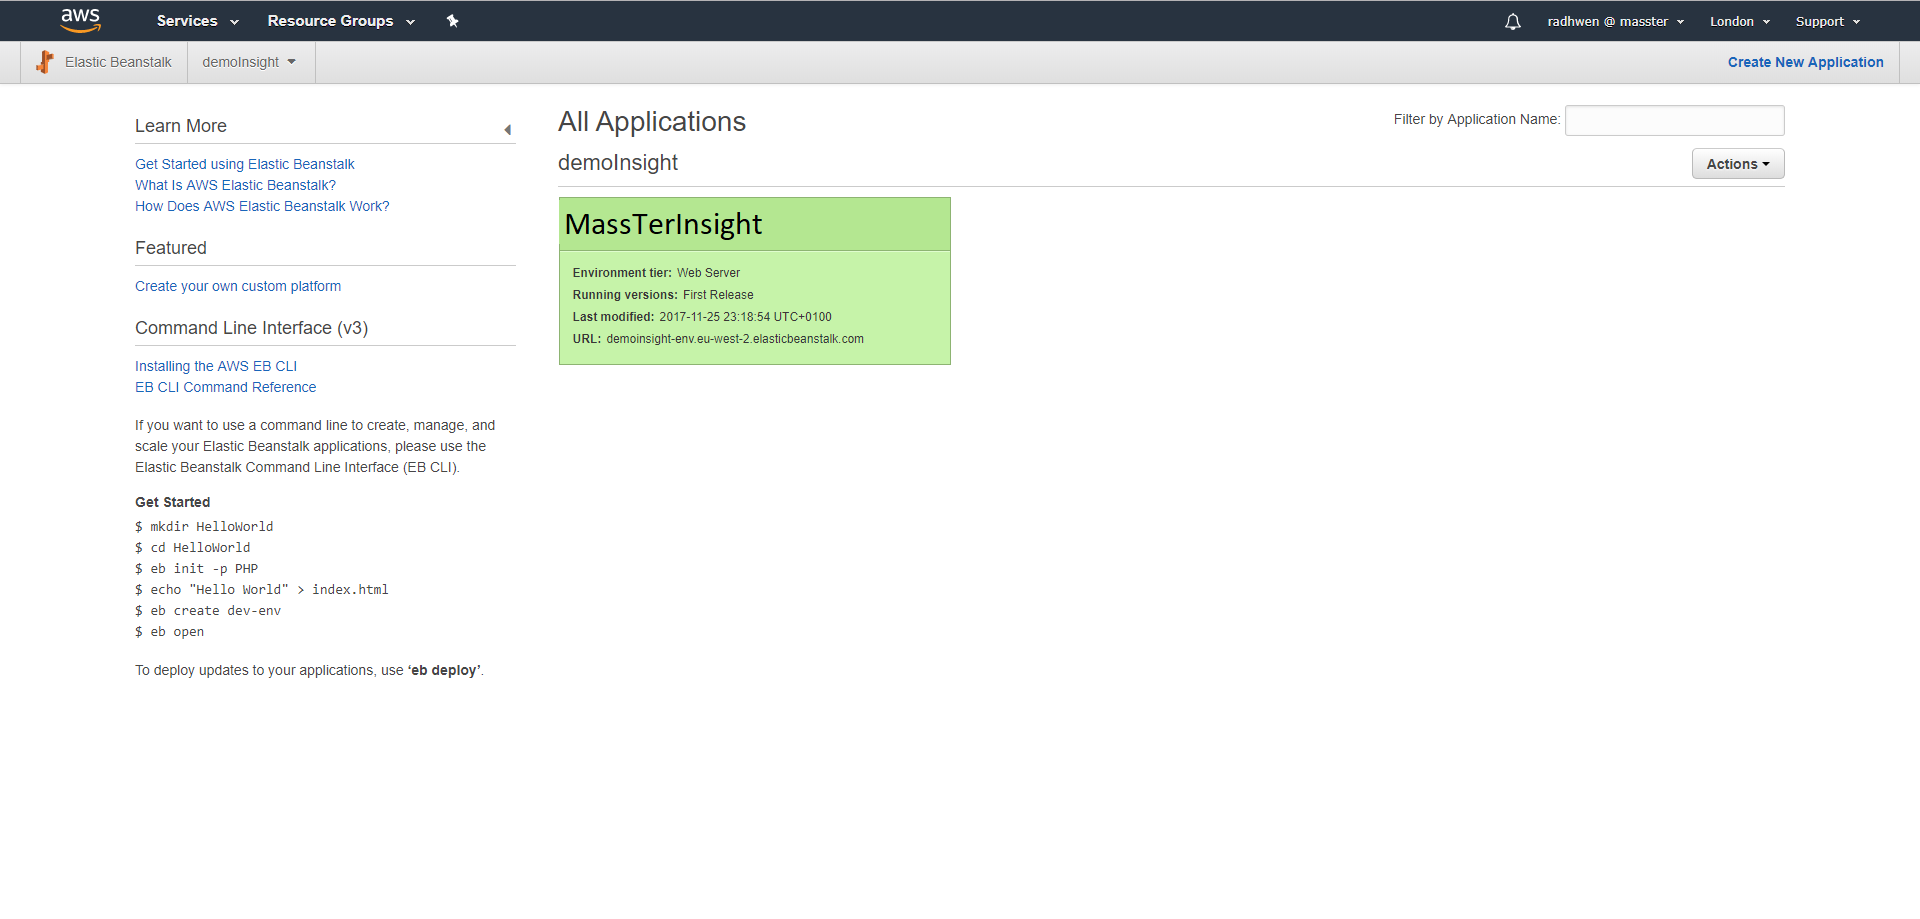
\includegraphics[width=17cm,height=10cm]{ElasticBeanstalkApplication.png}
		\caption{Elastic Beanstalk Application}	
	\end{figure}

After packaging our Web Application to .WAR using Apache MAVEN, then we deployed this package in Elastic beanstalk, the platform were the application is running is Tomcat.

After the deployment is done successfully, elastic beanstalk provides a URL for our application to be accessible in the INTERNET.
	 \begin{figure}[!h]
	\centering
	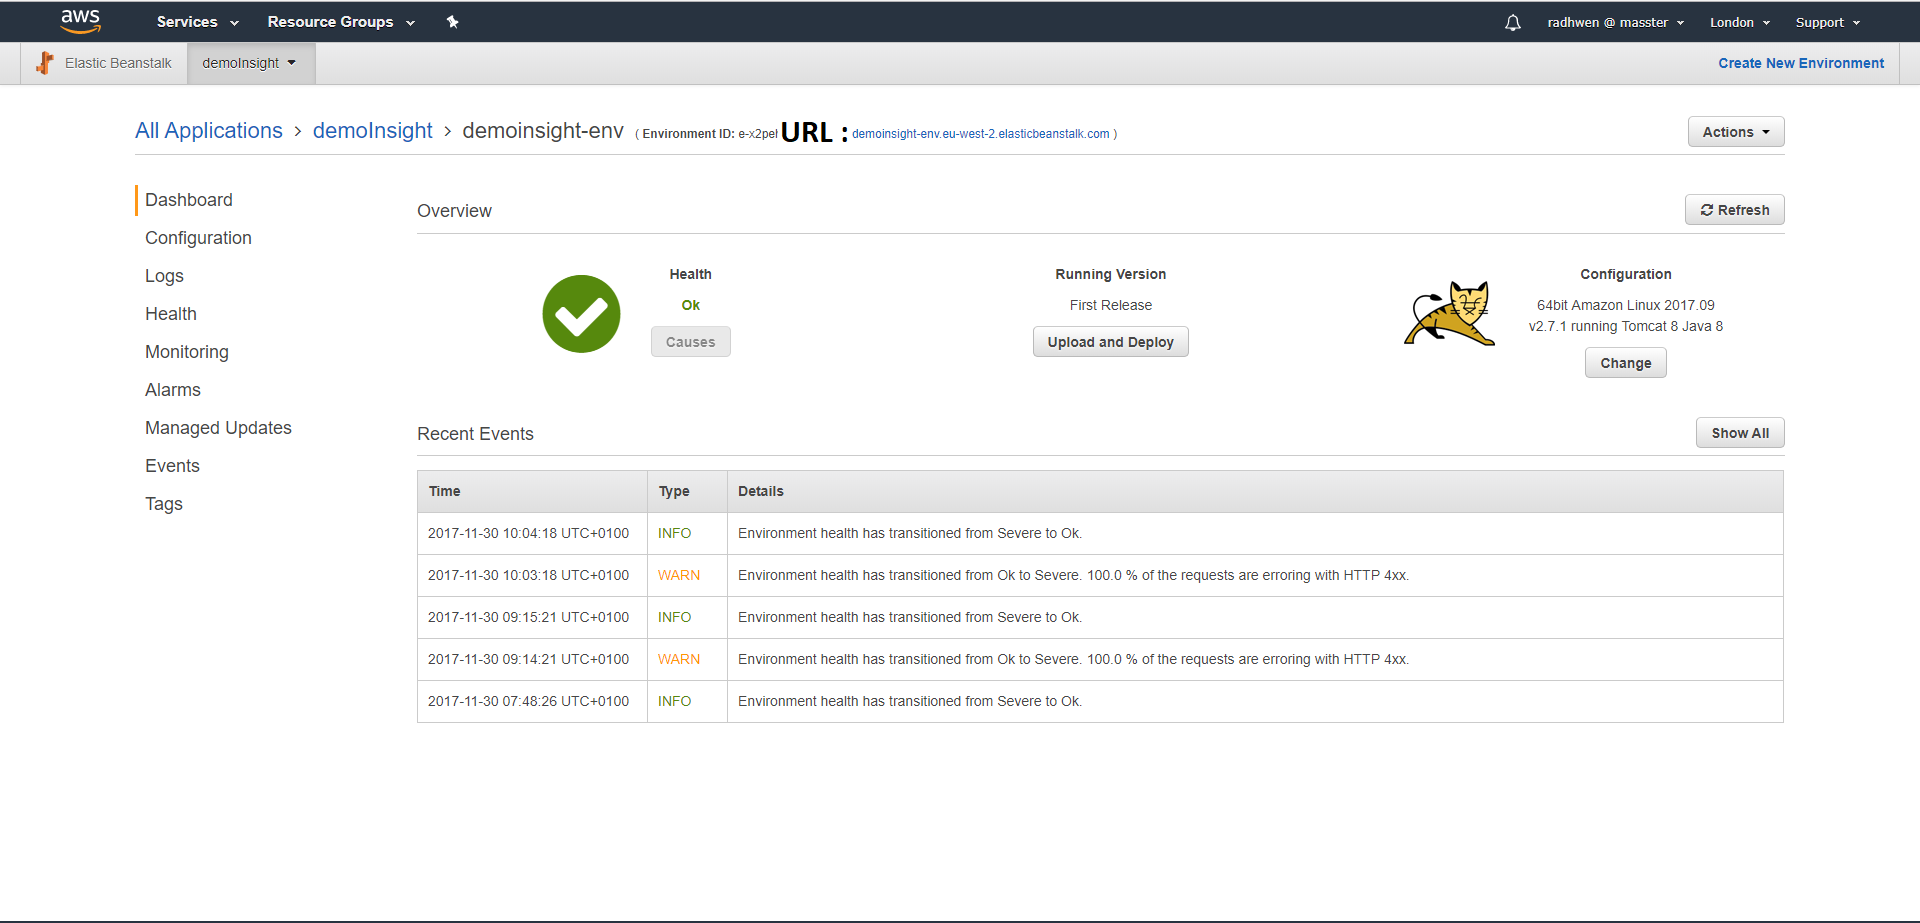
\includegraphics[width=17cm,height=9cm]{massTerInsightDashboard.png}
	\caption{MassTer Insight web Application Dashboard}	
\end{figure} 
	 \begin{figure}[!h]
	\centering
	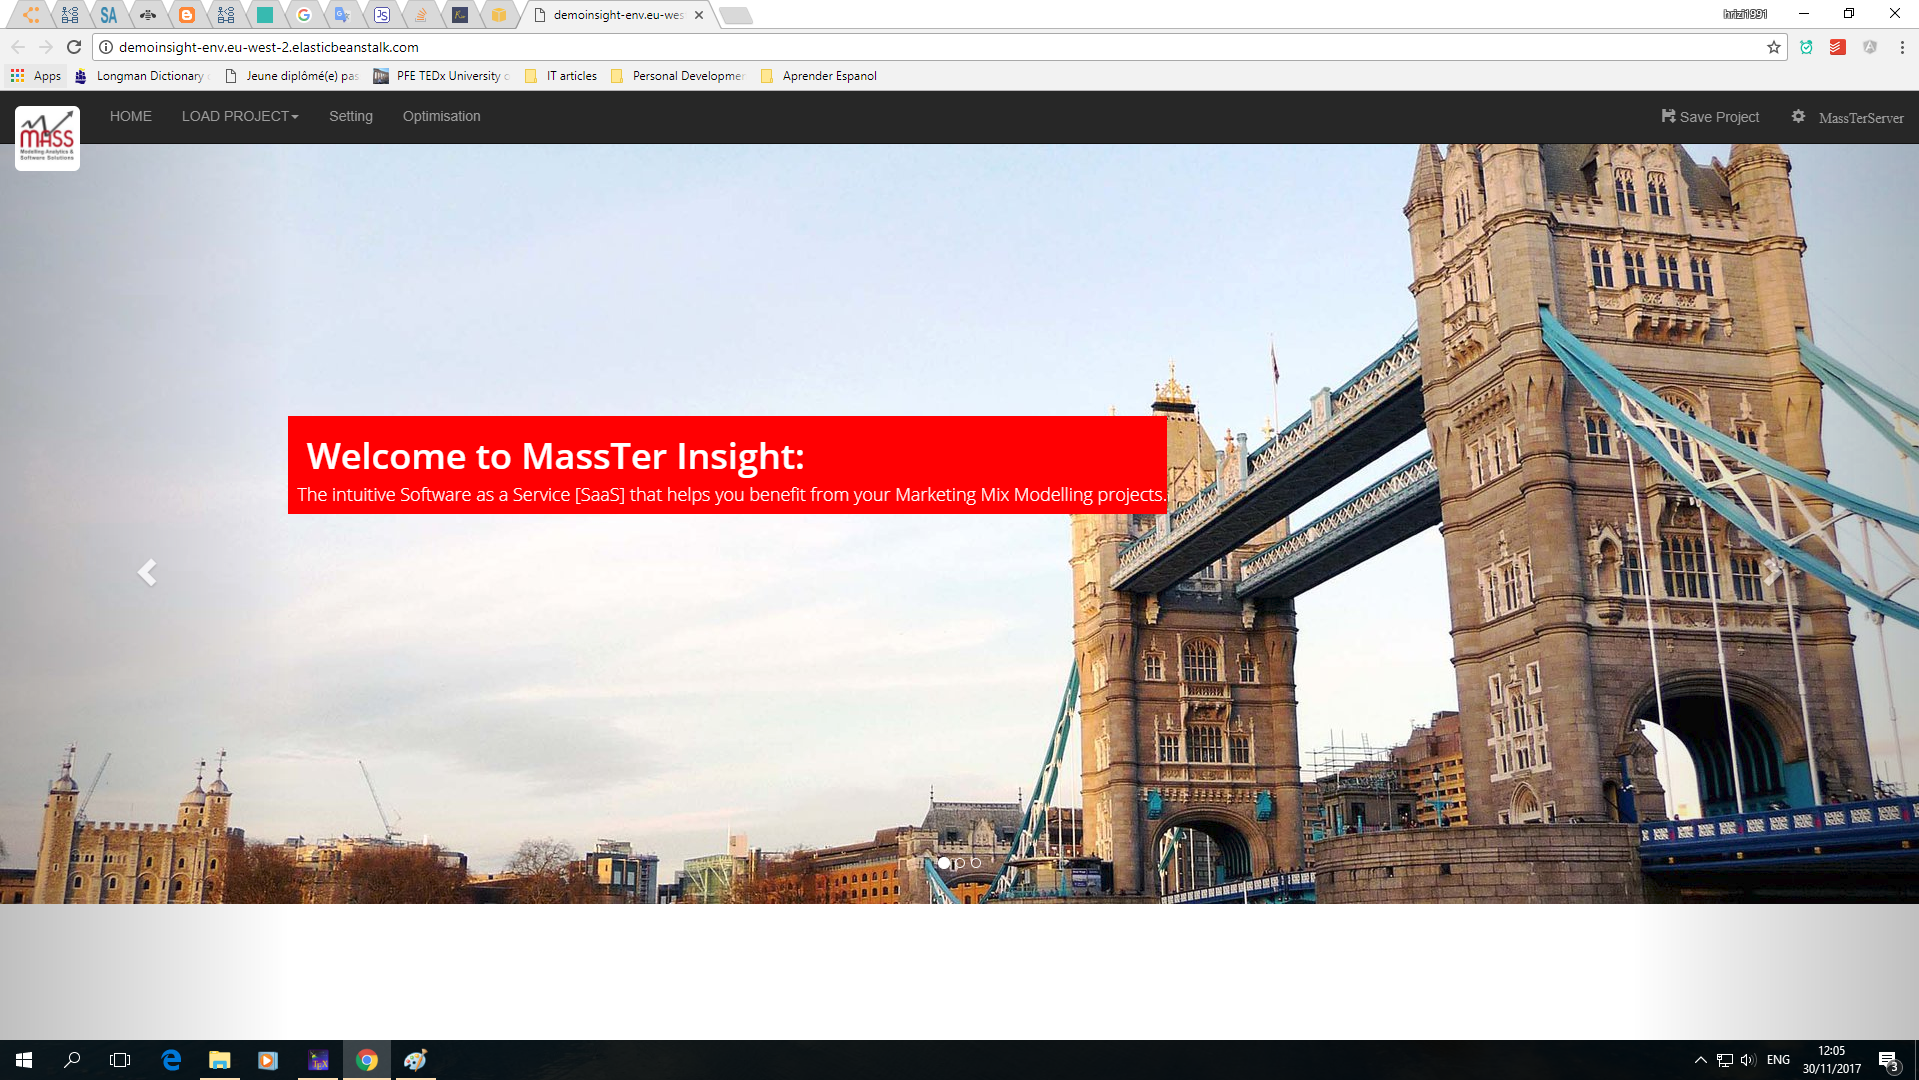
\includegraphics[width=17cm,height=9cm]{massTerInsightWeb.png}
	\caption{MassTer Insight web Application}	
\end{figure} 
     \clearpage
	\newpage 
	\subsection{Elastic Compute Cloud}
	Amazon EC2 is an \textbf{IaaS} offering from AWS. Amazon takes the responsibility of networking, storage, server and virtualization and the user is responsible for managing the operating System, midlleware, runtime, data and application.
	

	 \begin{figure}[!h]
		\centering
		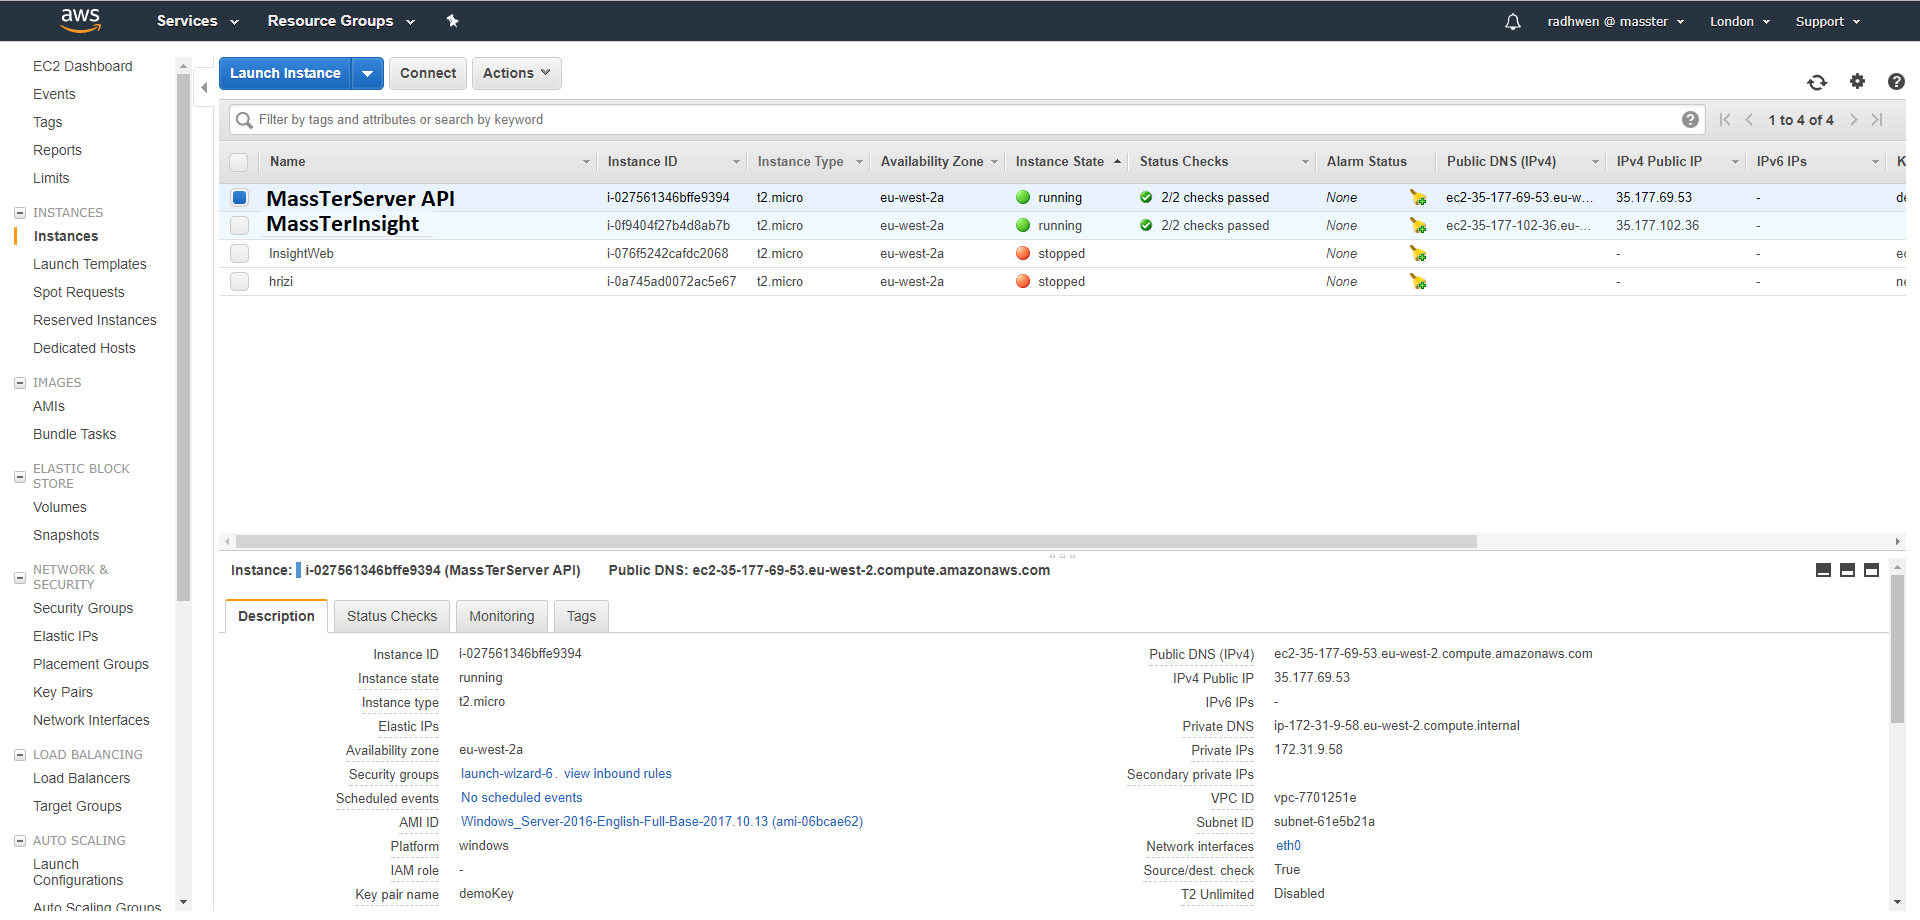
\includegraphics[width=17cm,height=9cm]{ec2Instance.png}
		\caption{EC2 Instance}	
	\end{figure} 

	MassTer Server API is running on EC2 Instance, we have chosen Windows Server 2016 as operating System, RAM 1Go, 30 Go Storage. 

	\section{Conclusion}
	In this chapter we present the way we deployed MassTer Server API and MassTer Insight, as a big achievement in this Internship is we  deployed The API MassTer Server and MassTer Insight Web Application successfully Using Amazon Web Services and now our Application Ready to be used through the Internet.